\documentclass[border=3pt]{standalone}
\usepackage{siunitx}
\usepackage[compat=1.1.0]{tikz-feynman}
\usepackage{amsmath, mathtools}
\begin{document}


\begin{minipage}[h]{0.25\linewidth}
	\centering
	\feynmandiagram [horizontal=a to b] {
	  i1 [particle=\(u\)] -- [fermion] a -- [fermion] i2 [particle=\(\bar{u}\)],
	  a -- [photon] b,
	  f1 [particle=\(\bar{t}\)] -- [fermion] b -- [fermion] f2 [particle=\(t\)],
	};
\end{minipage}

\hspace{0.15\linewidth}

\begin{minipage}[h]{0.15\linewidth}
	\centering
	\feynmandiagram [vertical=a to b] {
	  i1 [particle=\(g\)] -- [gluon] a -- [fermion] i2 [particle=\(t\)],
	  a -- [anti fermion] b,
	  f1 [particle=\(\bar{t}\)] -- [fermion] b -- [gluon] f2 [particle=\(g\)],
	};
\end{minipage}

\hspace{0.15\linewidth}

\begin{minipage}[h]{0.10\linewidth}
	\centering
	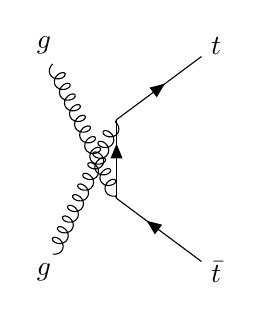
\begin{tikzpicture}
	  \begin{feynman}[small]
	    \vertex (a);
	    \vertex [below      =of a] (b);
	    \vertex [above left =of a] (i1) {\(g\)};
	    \vertex [below left =of b] (i2) {\(g\)};
	    \vertex [right      =of i2] (ff1);
	    \vertex [right      =of i1] (ff2);
		\vertex [right      =of ff1] (f1) {\(\bar{t}\)};
	    \vertex [right      =of ff2] (f2) {\(t\)};

	    \diagram* {
	      (i1) -- [gluon] (b)
	           -- [anti fermion] (f1),
	      (a) -- [anti fermion] (b),
	      (i2) -- [gluon] (a),
	      (a) -- [fermion] (f2),
	    };
	  \end{feynman}
	\end{tikzpicture}
\end{minipage}

\hspace{0.15\linewidth}

\begin{minipage}[h]{0.40\linewidth}
	\centering
	\feynmandiagram [horizontal=a to b] {
		i1 [particle=\(g\)] -- [gluon] a -- [gluon] i2 [particle=\(g\)],
		a -- [photon] b,
		f1 [particle=\(t\)] -- [anti fermion] b -- [anti fermion] f2 [particle=\(\bar{t}\)],
	};
\end{minipage}

\end{document}
